\chapter{Testentwurf}

Wie zuvor gesehen kann ein GraphQL-Schema mit Graphcoverage-Kriterien überdeckt werden.
Wir wollen diese Gegebenheit nun nutzen um eine Methode zur Generierung von Integrationstests für GraphQL zu entwickeln.
Hierbei werden wir uns in einigen Teilen an der Methode von \cite[Property-based Testing of GraphQL-APIs]{property-based-testing} bedienen.
Allerdings werden auch deutliche Unterschiede existieren.
Zuerst werden wir unsere Methode entwickeln und dann folgt ein Vergleich mit der Methode aus \cite[Property-based Testing of GraphQL-APIs]{property-based-testing}

\section{Schema in Graph abbilden}

Unser Ziel ist es, dass Wissen aus $5.2$ anzuwenden und mithilfe von Graphcoverage die Test zu generieren.
Hierfür benötigen wir erstmal einen Graphen, den wir untersuchen wollen.
Mithilfe der Introspection-Query kann von einer GraphQL-API das komplette Schema mit seinen Types abgefragt werden.
Die \hyperref[introspection-query]{Introspection-Query} ermöglicht es uns, dieses Schema von einer API abzufragen.
Hierbei ist zu beachten, dass nicht alle APIs dies unterstützen da einige diese Funktion ausgeschaltet haben oder
ein Depth-Limit in der Anfrage implementieren und die Anfrage zu komplex ist.
Beides vernachlässigen wir in unserer Methode da im Entwicklungskontext solche Maßnahmen weggelassen werden können.
Stellt man nun die \hyperref[introspection-query]{Introspection-Query} an eine GraphQL-API so hat die Response immer auch
die erwartete Struktur.
Im besonderen bedeutet das für uns, dass wir ein JSON-Objekt mit dieser Struktur bekommen:

\begin{lstlisting}[language=json, caption={Schema-Response},captionpos=b]
    {
        "data": {
            "__schema": {
                "queryType": {},
                "mutationType": {},
                "subscriptionType": {},
                "types": [],
                "directives": []
            }
        }
    }
\end{lstlisting}

Bei den Feldern $queryType$ , $mutationType$ und $subscriptionType$ wird jeweils ein Objekt erwartet.
Wobei wir hier mit der \hyperref[introspection-query]{Introspection-Query} nur den namen dieser Felder abfragen.
Diese Felder sind nämlich, wie in $4.2.2$ festgestellt grundlegende Typen eines jeden GraphQL-Schemas
können aber unter Umständen $null$ sein oder von den vordefinierten Namen $Query$, $Mutation$ und $Subscription$ abweichen.
Um solche Abweichungen abzufangen, werden diese mit abgefragt.
Im Feld $types$ finden wir dann alle möglichen Typdefinitionen.
Hierbei ist das Feld $types$ eine Liste, die alle definierten Typen des Schemas enthält.
Dies beinhaltet sowohl Custom-Types als auch die eingebauten Skalaren Datentypen.
Ein einzelner Type ist wie folgt definiert:

\begin{lstlisting}[language=json, caption={Type-Field},captionpos=b]
        {
          "kind": "",
          "name": "",
          "description": "",
          "fields": [],
          "inputFields": [],
          "interfaces": [],
          "enumValues": [],
          "possibleTypes": []
        }
\end{lstlisting}

Um nun aus dem Schema einen Graphen zu erstellen, benötigen wir die Felder $kind$, $name$, $fields$.
$kind$ ist die Angabe, von welchem Typ das Feld ist.
Hierbei gibt es 9 Möglichkeiten, die dieses Feld annehmen kann.

\begin{itemize}
    \item \textbf{ObjectTypeDefinition (OBJECT):} Repräsentiert ein Objekt mit Feldern.
    \item \textbf{ScalarTypeDefinition (SCALAR):} Eingebaute oder benutzerdefinierte Typen wie \texttt{Int}, \texttt{Float}, \texttt{String}, \texttt{Boolean} und \texttt{ID}.
    \item \textbf{InputObjectTypeDefinition (INPUT\_OBJECT):} Erlaubt das Übergeben komplexer Objekte als Argumente.
    \item \textbf{InterfaceTypeDefinition (INTERFACE):} Repräsentiert eine Liste von Feldern, die andere Objekttypen enthalten müssen.
    \item \textbf{UnionTypeDefinition (UNION):} Kann einen von mehreren Arten von Objekttypen repräsentieren.
    \item \textbf{EnumTypeDefinition (ENUM):} Ein Skalartyp, der auf eine bestimmte Liste von Werten beschränkt ist.
    \item \textbf{ListTypeDefinition (LIST):} Repräsentiert eine Liste von Werten eines bestimmten Typs.
    \item \textbf{NonNullTypeDefinition (NON\_NULL):} Ein Modifikator, der angibt, dass der angewandte Typ nicht null sein kann.
    \item \textbf{DirectiveDefinition (DIRECTIVE):} Passt das Verhalten von Feldern oder Typen  Schema an.
\end{itemize}

Um einen Graphen aus dem Schema zu entwickeln benötigen wir nur Felder vom Typ $OBJECT$.
Die Menge aller Objekte vom Typ $OBJECT$ sind die Menge aller Knoten unseres Graphens.
Um nun die Kanten, also die Beziehungen zwischen diesen einzelnen Knoten zu bekommen müssen wir uns die Defintion
eines Typens näher ansehen.
Wie in $Type-Field$ gesehen, definiert ein Type immer ein Feld $fields$.
In diesem Feld $fields$ verbirgt sich die Informationen aller Kanten, die ausgehend von diesem Knoten sind.
Das Feld $fields$ beeinhaltet Objekte folgender Struktur:

\begin{lstlisting}[language=json, caption={Type-Field},captionpos=b]
            {
              "name": "",
              "description": "",
              "args": [],
              "type": {},
              "isDeprecated": "",
              "deprecationReason": ""
            }
\end{lstlisting}

Wobei für die Kantensuche das Feld type besonders wichtig ist.
Dieses ist wie folgt definiert:

\begin{lstlisting}[language=json, caption={Type-Field},captionpos=b]
    {
        "kind": "",
        "name": "",
        "ofType": null
    }
\end{lstlisting}

Wenn nun der Eintrag $kind$ den Wert $OBJECT$ trägt, so ist klar, dass unser hier definiertes $OBJECT$ eine Kante zum
Knoten $name$ besitzt.
Man kann nun einmal über alle Einträge von $types$ gehen und jeden Eintrag vom Typ $OBJECT$ als Knoten anlegen.
In einem zweiten Durchlauf kann man dann über alle $fields$ von jedem Type gehen und die Kanten zwischen den Knoten ziehen.
Hierzu folgt nun noch ein minimales Beispiel eines sehr kleinen Schemas und das Mapping zum dazugehörigen Graphen.
Wir werden hierbei Schritt für Schritt vorgehen.
Zuerst definieren wir ein GraphQL-Schema:

\begin{lstlisting}[ caption={Schema Definition},captionpos=b]
  type Query {
    book(id: ID): Book
    author(id: ID): Author
    publisher(id: ID): Publisher
  }

  type Book {
    id: ID
    title: String
    author: Author
    publisher: Publisher
  }

  type Author {
    id: ID
    name: String
    books: [Book]
  }

  type Publisher {
    id: ID
    name: String
    books: [Book]
  }
\end{lstlisting}

Für dieses Schema erhalten wir dann eine JSON-Response zurück im Format wie in 6.1 vorgestellt.
Die vollständige Response ist in \hyperref[minimal-schema-response]{minimale Schema Response} zu finden.
In dieser Response werden 4 Typen vom Typ $OBJECT$ definiert, diese sind wie erwartet unsere eben definierten types
$Query$, $Book$, $Author$ und $Publisher$.
Durch die erste Iterierung können wir also nun folgern, dass unser zu erstellende Graph 4 Knoten besitzen muss.

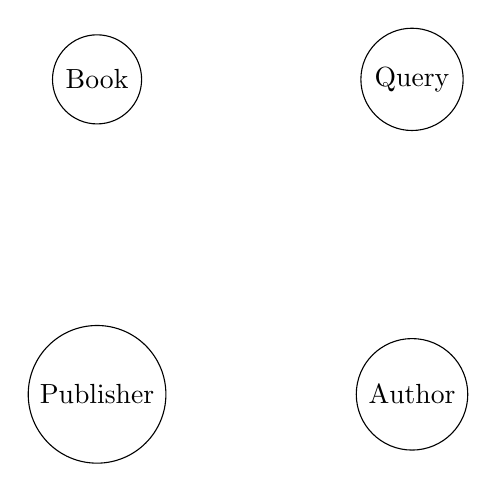
\begin{tikzpicture}
  \node[circle, draw] (n1) at (4,4) {Query};
  \node[circle, draw] (n2) at (0,4) {Book};
  \node[circle, draw] (n3) at (4,0) {Author};
  \node[circle, draw] (n4) at (0,0) {Publisher};
\end{tikzpicture}

In einer zweiten Iteration prüfen wir nun alle $fields$ Einträge des jeweiligen Types die vom Typ $OBJECT$ sind.
Beginnend im Query Type finden wir dort 3 Einträge in $fields$.
Jedes Feld besitzt einen Namen, in diesem Beispiel sind dies $book$, $author$ und $publisher$.

\begin{lstlisting}[language=json, caption={book Field},captionpos=b]
            {
              "name": "book",
              "description": null,
              "args": [
                {
                  "name": "id",
                  "description": null,
                  "type": {
                    "kind": "SCALAR",
                    "name": "ID",
                    "ofType": null
                  },
                  "defaultValue": null
                }
              ],
              "type": {
                "kind": "OBJECT",
                "name": "Book",
                "ofType": null
              },
              "isDeprecated": false,
              "deprecationReason": null
            }
\end{lstlisting}

\begin{lstlisting}[language=json, caption={author Field},captionpos=b]
            {
              "name": "author",
              "description": null,
              "args": [
                {
                  "name": "id",
                  "description": null,
                  "type": {
                    "kind": "SCALAR",
                    "name": "ID",
                    "ofType": null
                  },
                  "defaultValue": null
                }
              ],
              "type": {
                "kind": "OBJECT",
                "name": "Author",
                "ofType": null
              },
              "isDeprecated": false,
              "deprecationReason": null
            }
\end{lstlisting}

\begin{lstlisting}[language=json, caption={publisher Field},captionpos=b]
            {
              "name": "publisher",
              "description": null,
              "args": [
                {
                  "name": "id",
                  "description": null,
                  "type": {
                    "kind": "SCALAR",
                    "name": "ID",
                    "ofType": null
                  },
                  "defaultValue": null
                }
              ],
              "type": {
                "kind": "OBJECT",
                "name": "Publisher",
                "ofType": null
              },
              "isDeprecated": false,
              "deprecationReason": null
            }
\end{lstlisting}

Eine gerichtete Kante muss nun ausgehend vom Query-Knoten gezogen werden jeweils zum $type$ jedes einzelnen Feldes.
Die Kante erhält als Gewicht hierbei dann exakt die Feld-Definition.
So wird es später möglich aus Pfaden Querys zu bilden.
Nachdem alle Knoten iteriert wurden und die Felder untersucht sind, ergibt sich folgender Graph für unser Schema:

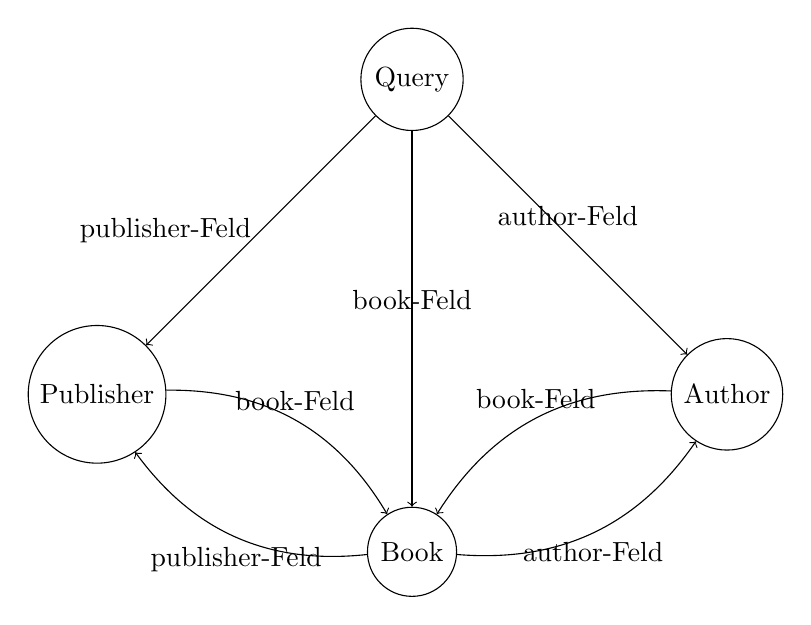
\begin{tikzpicture}
    \node[circle, draw] (n1) at (8,6) {Query};
    \node[circle, draw] (n2) at (8,0) {Book};
    \node[circle, draw] (n3) at (12,2) {Author};
    \node[circle, draw] (n4) at (4,2) {Publisher};

    \draw[->] (n1) -- node[above] {book-Feld} (n2);
    \draw[->] (n1) -- node[above] {author-Feld} (n3);
    \draw[->] (n1) -- node[left]  {publisher-Feld} (n4);
    \draw[->] (n2) to[bend right] node[below] {author-Feld} (n3);
    \draw[->] (n3) to[bend right] node[above] {book-Feld} (n2);
    \draw[->] (n2) to[bend left]  node[below] {publisher-Feld} (n4);
    \draw[->] (n4) to[bend left]  node[above] {book-Feld} (n2);
\end{tikzpicture}

Aus diesem Graphen können wir nun unsere Tests entwickeln.
Hierzu in den folgenden Kapiteln mehr.

\section{Pfade aus Graph bilden}

Dieser Schritt ist optional, je nach Implementation der Algorithmen für die Graphüberdeckung.
Es ist hierbei möglich einen generativen oder filternden Ansatz zu verfolgen.
Wird ein generativer Ansatz verfolgt, so wird direkt $6.3$ angewandt.
Alternativ generieren wir erstmal alle möglichen Simple-Paths (noch definieren - TODO) ausgehend von einem Startknoten.
Wir müssen die Simple-Paths vom Startknoten generierien, da in GraphQL nur Anfragen erlaubt sind, die in diesem Startknoten
beginnen.
Im allgemeinen Fall ist dies der Knoten $Query$
Diese Simple-Paths werden dann im nächsten Schritt gefiltert durch das jeweilige Coverage-Kriterium.
In unserem Beispielgraphen sind die Simple-Paths folgende:

\begin{itemize}
    \item (Query, Book)
    \item (Query, Author)
    \item (Query, Publisher)
    \item (Query, Author, Book)
    \item (Query, Publisher, Book)
    \item (Query, Book, Author)
    \item (Query, Book, Publisher)
    \item (Query, Publisher, Book, Author)
    \item (Query, Author, Book, Publisher)
\end{itemize}

\section{Coverage-Pfade ermitteln}

Wie zuvor unterschieden, gibt es zwei Verfahren um die Pfade zu generieren.
Wir werden hier beide Verfahren getrennt voneinander
Zuerst betrachten wir den filternden Ansatz da er thematisch zum vorherigen Kapitel abschließend ist.

\subsection{filternder Ansatz}
Aus der zuvor gewonnen Menge an Simple-Paths können wir nun je nach Coverage-Kriterium die Pfade, die für unser Coverage-Kriterium
wichtig sind, herausfiltern.
Exemplarisch nutzen wir hierfür einmal die Prime-Path Coverage.
Es ist jedoch denkbar auch andere Coverage-Kriterien zu verwenden.
Wir erinnern uns: Ein Prime-Path ist ein Pfad, der weder selbst Teil eines anderen Pfades ist noch sich wiederholt.
Dies bedeutet, dass wir alle Pfade aus den Simple-Paths danach filtern müssen, dass diese weder Teilpfad eines anderen Pfades sind
noch, dass sie sich wiederholen.
Hier kann man folgenden Pseudo-Code nutzen um einen Filter für PrimePaths zu entwickeln:

\begin{verbatim}
    Input: alle_Pfade

    prime_paths = []

    Für alle_Pfade:
        Wenn istPrimePfad(Pfad, alle_Pfade):
            prime-paths =+ Pfad
        Sonst verwerfe Pfad

    return prime_paths


    Funktion istPrimePfad(möglicherPrimePath, alle_Pfade):
        Für pfad in alle_Pfade:
            Wenn möglicherPrimePath != pfad and istTeilpfad(möglicherPrimePath, pfad)
                return False
        return True

    Funktion istTeilpfad(möglicherPrimePath, pfad):
        Wenn Länge(möglicherPrimePath) > Länge(pfad):
            return False
        Für jeden TeilPfad von Pfad:
            Wenn TeilPfad = möglicherPrimePath:
                return True
        return False

\end{verbatim}

Dieser PseudoCode bewirkt, dass wir für jeden Pfad ermitteln ob dieser ein PrimePath ist.
Hierbei iterieren wir über jeden einzelnen Pfad und prüfen ob dieser ein PrimePfad ist.
Hierbei fügen wir einen Pfad der Liste alle Prime-Paths hinzu, wenn dieser die Funktion istPrimePfad mit $True$ erfüllt.
Die Funktion liefert hierbei nur $True$ zurück, wenn der Pfad sich nicht wiederholt und er die Funktion istTeilpfad mit False belegt.
Somit erreichen wir genau, dass nur diejenigen Pfade mit $True$ in die Liste gegeben werden, die genau unsere eingangs definierten Bedinungen
erfüllen.
Nutzen wir nun diesen Pseudo-Code auf unserer Menge der SimplePaths so bekommen wir folgende PrimePaths:

\begin{itemize}
    \item (Query, Book, Author)
    \item (Query, Publisher, Book, Author)
    \item (Query, Book, Publisher)
    \item (Query, Author, Book, Publisher)
\end{itemize}

Diese filternde Methode ist im Allgemein einfacher zu implementieren, bietet jedoch einen großen Nachteil:
Die Generierung der SimplePaths ist sehr rechenintensiv und außerdem werden hierfür Pfade nur entfernt aus der größeren Menge.
Dies bedeutet, dass die SimplePaths eine schon sehr gute Abdeckung bieten und die PrimePaths den Testraum nur potentiell verkleinern da wir eben
nur aus der SimplePath Menge dann Pfade löschen.
Die Methode des Filterns eignet sich also am ehesten für kleine Schemas da hier das bilden der SimplePaths noch relativ rechenarm
ist und zur Validierung von verschiedenen CoverageKriterien da die generative Implementierung komplexer ist.
Hierdurch kann man also vorher überprüfen, ob es sich lohnt ein anderes CoverageKriterium mittels generativem Ansatz zu implementieren.
Der generative Ansatz gewinnt dann an Bedeutung wenn die GraphQL-Schemas größer werden da so Rechenzeit gespart werden kann.
Es sei außerdem erwähnt, dass die Ausführungszeit der Tests auch relevant sein kann und somit die Anzahl an Pfaden durch Filtern reduziert werden muss.

\subsection{generativer Ansatz}

Mittels eines generativen Ansatzes lassen sich von einem gegebenen Startpunkt die Pfade ermitteln, welche die gewünschte Coverage
erreichen.
Hierbei unterscheidet sich der konkrete Ansatz je nach Coverage-Kriterium wieder.
Im allgemeinen wird eine Funktion $generatePaths(Startpunkt, Graph)$ erwartet.
Wobei der Startpunk im Allgemeinen der $Query$ Knoten ist und $Graph$ den kompletten Graphen abbildet.
Erwarteter Rückgabewert der Methode ist eine Liste von Pfaden die das jeweilige CoverageKriterium erfüllen.
Wir werden auch hier wieder einen Pseudo Code vorstellen, der für die Generierung von Prime-Paths zuständig ist aber allerdings
den generativen Ansatz verfolgt.

\begin{verbatim}

    testPfade = []
    Generiere_Prime_Pfade(startknoten, [], testPfade, Graph)


    Function Generiere_Prime_Pfade(Knoten, Pfad, testPfade, Graph):
        Füge den Knoten dem Pfad hinzu
        Für alle FolgeKnoten von Knoten:
            Wenn FolgeKnoten nicht in Pfad:
                generiere_Prime_Pfade(FolgeKnoten, testPfade, Pfadliste, Graph)
        Wenn Ist_PrimePfad?(Pfad, testPfade):
            Füge Pfad den testPfaden hinzu

    Function Ist_PrimePfad?(neuerPfad, testPfade):
        Für alle Pfade in TestPfade:
            Wenn neuerPfad ein Teilpfad eines Pfades ist
                return False
        return True

\end{verbatim}

Der Pseudocode startet im Startpunkt des Graphens und iterriert dann rekursiv über die Folgeknoten des Graphens.
Hierbei wird stets in Beachtung gehalten, dass ein Knoten in einem Pfad nicht zweimal vorkommen kann.
So vermeiden wir Kreise und eine mögliche, unendlichen Generierungsraum.
Für jeden generierten Pfad wird dann überprüft ob dieser ein Prime-Path ist.
Dies ist der Fall wenn er kein Teilpfad eines anderen Pfades ist und sich nicht selbst wiederholt.
Wir stellen sicher, dass der Pfad sich nicht wiederholen kann indem wir Kreise erst gar nicht zulassen.
Im zweiten Schritt prüfen wir dann ob ein Pfad ein Teilpfad ist.
Endergebniss sind dann die Prime-Paths des Graphens.
Dieser Code ergibt dann folgende Pfade für die PrimePath-Coverage die den Graphen überdecken:

\begin{itemize}
    \item (Query, Book, Author)
    \item (Query, Publisher, Book, Author)
    \item (Query, Book, Publisher)
    \item (Query, Author, Book, Publisher)
\end{itemize}

Wir sehen diese sind identisch zum filternden Ansatz.

\section{Query aus Pfad ermitteln}

Da wir nun die Pfade, je nach Coveragekriterium ermittelt haben müssen wir nun eine Query aus diesen Pfaden bilden.
Hierbei nutzen wir diverse Hinweise die im GraphQL-Schema gegeben werden und einen Teil der Arbeit aus \cite[Property-Based Testing]{property-based-testing}.
Jeder ermittelte Pfad startet im Query-Knoten.
Da wir zuvor den Kanten jeweils die Feldattribute mitgegeben haben, können wir nun sehr einfach ermitteln welche
Operationen wir ausführen müssen, um von einem Knoten zum nächsten zu kommen.
Dies bedeutet, dass die Kanteninformationen ausreichen, um eine Query zu bilden.
Wir gehen hierbei den kompletten Pfad ab und geben einen Query-String zurück der für GraphQL zulässig ist.
Eine valide GraphQL-Query beginnt mit $\{ \}$ und folgt dann mit der ersten Felddefinition.
Eine Felddefinition kann vom Type $SCALAR$ oder $OBJECT$ sein.
Ist ein Feld vom Type $SCALAR$ so kann dieses einfach der Query hinzugefügt werden als erwartetes Feld.
GraphQLs Spezialität ist es, dass nur wirklich angeforderte Felder in einer Response existieren.
Im Kontext des Integrationstesten wollen wir aber alle möglichen Felder abfragen einfach um sicher zu gehen, dass
diese korrekt Installiert wurden.
Es wäre denkbar auch Variationen der einzelnen Felder zu implementieren, dass nicht in jeder Query immer alle Felder
eines Typen berücksichtig werden, dies wird hier jedoch zuerst vernachlässigt und wir inkludieren alle Felder.
Ist ein Feld vom Type $OBJECT$ so bedeutet dies, dass dieses Feld nur angegeben werden muss, wenn der nachfolgende Knoten im Pfad
exakt den Typen dieses Feldes hat!
Das Feld wird dann wieder eingeleitet durch $\{ \}$.
Innerhalb dieser Felder ist nun wieder jedes Feld des Typen $SCALAR$ hinzuzufügen und das Feld des nächsten Knotens zu suchen sowie hinzuzufügen.
Sollte ein Feld vom Type $OBJECT$ Argumente benötigen, so steht dies im Schema und wir können diese generieren.
Input-Argumente können vom Type $INPUT-OBJECT$ sein oder $SCALAR$.
Sollte es ein Scalar Type sein, so bedienen wir uns der Methode aus \cite[Property-based Testing]{property-based-testing} und generieren
jeweils Zufallsargumente in Form des jeweiligen Datentyps.
Sollte das Argument vom Type $INPUT-OBJECT$ sein so lässt es sich in seine Bestandteile zerlegen welche auch wieder $SCALAR$ Types sind und
dann werden diese auch zufällig entsprechend generiert und dem $INPUT-OBJECT$ Type entsprechend angeordnet.
Argumente folgen dann jeweils zwischen dem Namen des Felds vom $OBJECT$ und den sich öffnenden, geschweiften Klammern.
Für unser Beispiel von vorher bedeutet dies also, dass wenn wir aus dem Pfad $(Query, Book, Publisher)$ eine Query bilden wollen, wir folgende
Schritte zu erfüllen haben:

\begin{enumerate}
    \item Finde Kante von $Query$ zu $Book$
    \item Ermittel ob die Kante $(Query, Book)$ Argumente benötigt.
    \item Ermittel alle $SCALAR$ Types die $Book$ definiert.
    \item Ermittel die Kante von $Book$ zu $Publisher$
    \item Ermittel ob die Kante $(Book, Publisher)$ Argumente benötigt.
    \item Ermittel alle $SCALAR$ Types die $Publisher$ definiert
    \item Baue Query-String aus den erlangten Informationen
\end{enumerate}


Wir werden nun Schritt für Schritt alle Schritte einzeln durchgehen und unsere Query generieren.

\begin{minipage}[t]{0.5\textwidth}
    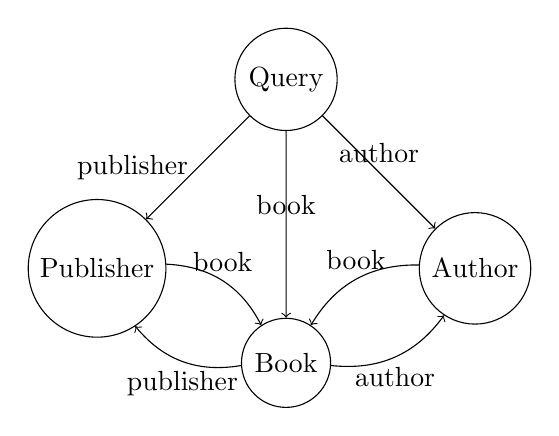
\begin{tikzpicture}[scale=0.6, baseline=(current bounding box.north)]
        \node[circle, draw] (n1) at (8,6) {Query};
        \node[circle, draw] (n2) at (8,0) {Book};
        \node[circle, draw] (n3) at (12,2) {Author};
        \node[circle, draw] (n4) at (4,2) {Publisher};

        \draw[->] (n1) -- node[above] {book} (n2);
        \draw[->] (n1) -- node[above] {author} (n3);
        \draw[->] (n1) -- node[left]  {publisher} (n4);
        \draw[->] (n2) to[bend right] node[below] {author} (n3);
        \draw[->] (n3) to[bend right] node[above] {book} (n2);
        \draw[->] (n2) to[bend left]  node[below] {publisher} (n4);
        \draw[->] (n4) to[bend left]  node[above] {book} (n2);
    \end{tikzpicture}
\end{minipage}%

\begin{minipage}[t]{0.5\textwidth}
    \vspace{0.5cm}



\end{minipage}









\section{Test ausführen \& Testauswertung}

\section{Zusammenfassung der Methode}

\section{struktureller Vergleich mit Property-based Testing}
